%%%%%%%%%%%%%%%%%%%%% MENU PRINCIPAL %%%%%%%%%%%%%%%%%%%%%%%%
\section{Menú principal}

\paragraph{}
Desde el menú principal se podrá acceder a los distintos modos de juego disponibles en \emph{Zycars}, así
como las opciones del juegos y la información sobre los desarrolladores del proyecto.

\begin{figure}[H]
  \label{menu_princiapl}
  \begin{center}
    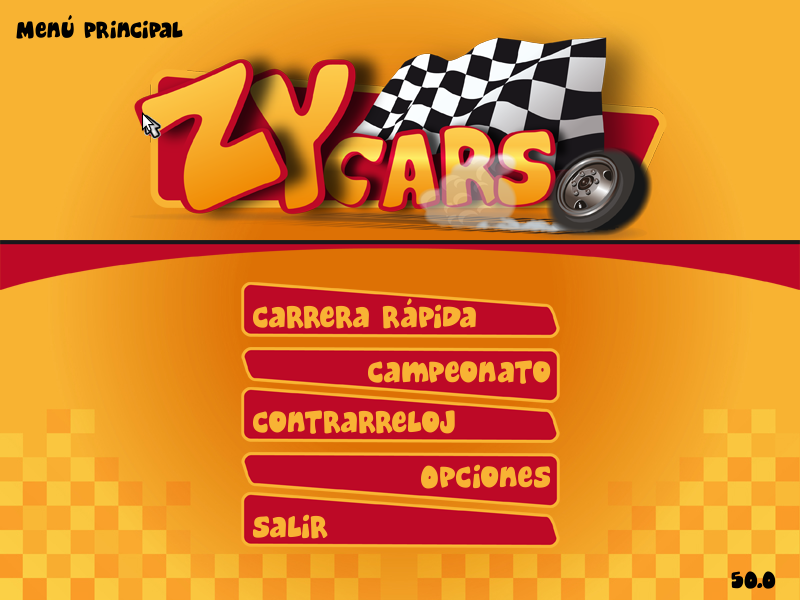
\includegraphics[scale=0.4]{imagenes/capturas/menuprincipal.png}
  \end{center}
  \caption{Manual de usuario: Menú principal}
\end{figure}

\paragraph{}
Debe usar el ratón para seleccionar la opcion que desee.

%%%%%%%%%%%%%%%%%%%% MODOS DE JUEGO %%%%%%%%%%%%%%%%%%%%%%%
\section{Modos de juego}

\paragraph{}
En \emph{Zycars} hay disponibles tres modos de juegos, en los que competiremos solos o contra la máquina en función
del objetivo que tengamos que lograr.

\subsection{Carrera rápida}

\paragraph{}
El modo carrera rápida consiste en competir contra la inteligencia artificial en una única carrera, con el objetivo de 
mejorar nuestras habilidades y acostumbrarse a los controles del juego. A lo largo del circuito podremos obtener distintos
items con los que hacer frente a nuestros competidores.

\subsection{Campeonato}

\paragraph{}
En el modo Campeonato competiremos contra la inteligencia artificial a lo largo de cuatro circuitos, en los que obtendremos
una puntuación en relación a la posición que hayamos obtenido al concluir la carrera, 4 puntos para el ganador, 2 puntos para
el segundo clasificado, 1 punto para el tercero y 0 puntos para el ultimo en concluir la carrera. El competidor que mas puntos haya 
conseguido al concluir el campeonato, será el ganador del mismo. En este modo también encontraremos items durante las distintas carreras.

\subsection{Contrarreloj}

\paragraph{}
En este modo de juego, el modo contrarreloj, el objetivo será batir los distintos records de tiempo que tienen cada uno de los 
circuitos, podremos mejorar tanto el tiempo general de la carrera, como el tiempo obtenido en la vuelta mas rápida. Tendremos
un máximo de 3 vueltas para mejorar los tiempos. En este modo de juego no encontraremos items, ya que no tendremos ningún oponente
al que tengamos que batir.


%%%%%%%%%%%%%%%%%% SELECCION DE PERSONAJE %%%%%%%%%%%%%%%%%%%%
\section{Menú de selección de personaje}

\paragraph{}
Una vez seleccionado un modo de juego, pasaremos al menú de seleccion de personaje. En este menú se nos mostrarán todos
los personajes disponibles en \emph{Zycars}, asi como el coche que cada uno de ellos conduce y las distintas características
que poseen los coches.

\begin{figure}[H]
  \label{menu_personaje}
  \begin{center}
    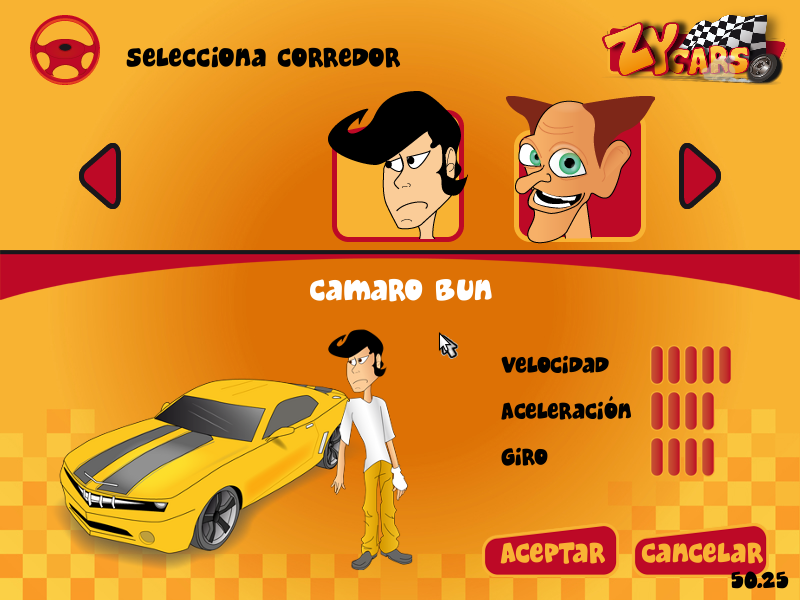
\includegraphics[scale=0.4]{imagenes/capturas/seleccionpersonaje.png}
  \end{center}
  \caption{Manual de usuario: Menú selección de personaje}
\end{figure}

\paragraph{}
Con el ratón podremos navegar sobre los distintos personajes pulsando sobre las flechas rojas. Pulsaremos en el botón
aceptar, para elegir el personaje seleccionado. Si queremos volver al menún principal, pulsaremos sobre el botón cancelar.

%%%%%%%%%%%%%%%%%% SELECCION DE CIRCUITO %%%%%%%%%%%%%%%%%%%%%
\section{Menú de selección de circuito}

\paragraph{}
Una vez seleccionado el personaje con el que deseamos competir, pasaremos al menú de selección de circuito. En este menú
se nos muestran los distintos campeonatos que posee el juego, así como los circuitos que componen cada uno de los 
campeonatos. 

\begin{figure}[H]
  \label{menu_circuito}
  \begin{center}
    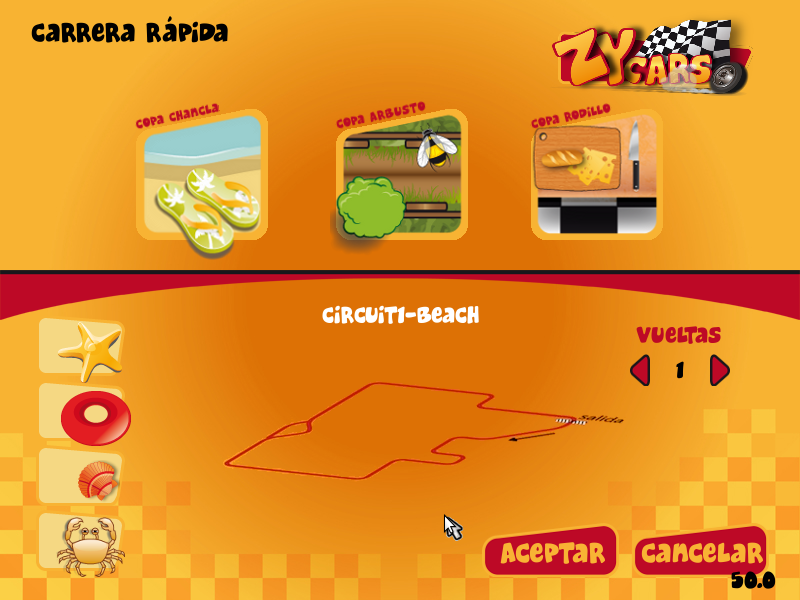
\includegraphics[scale=0.4]{imagenes/capturas/menucircuito.png}
  \end{center}
 \caption{Manual de usuario: Menú selección de circuito}
\end{figure}

\paragraph{}
Si nos encontramos en el modo carrera rápida o en el modo contrarreloj, deberemos seleccionar algún circuito de todos los
disponibles, una vez elejido, pulsaremos aceptar, en el caso de que queramos volver al menú de selección de personaje
pulsaremos sobre el botón cancelar.

\paragraph{}
Si estamos en el modo campeonato, podremos ver todos los circuitos que componen cada uno de los campeonato, al pulsar sobre
el botón aceptar, indicaremos que seleccionamos el campeonato actual. Si pulsamos el botón cancelar volveremos al menú de selección
de personaje.

\paragraph{}
Podremos elegir, en la parte derecha del menú, el número de vueltas que queremos que realicen en cada una de las carreras. Esta opción
no estará disponible en el modo campeonato, ya que en este modo siempre habra que dar 3 vueltas al circuito.

%%%%%%%%%%%%%%%%%% OPCIONES %%%%%%%%%%%%%%%%%%%%%%
\section{Menú de Opciones}

\paragraph{}
En el menú de opciones, podremos modificar distintos apartados como sonido, características de pantalla y controles del juego. 
Una vez realizados los cambios y deseamos que se apliquen debemos pulsar el botón aceptar, si por el contrario deseamos volver al
menú principal si que se aplique ninguno de los cambios realizados, debemos pulsar sobre el botón cancelar.

\subsection{Sonido}

\paragraph{}
En este menú podremos seleccionar y modificar tanto el volumen de los efectos de sonido que se encuentran en el juego, así 
como el volumen de la música que escuchamos a lo largo de las distintas pantallas y circuitos.

\begin{figure}[H]
  \label{menu_audio}
  \begin{center}
    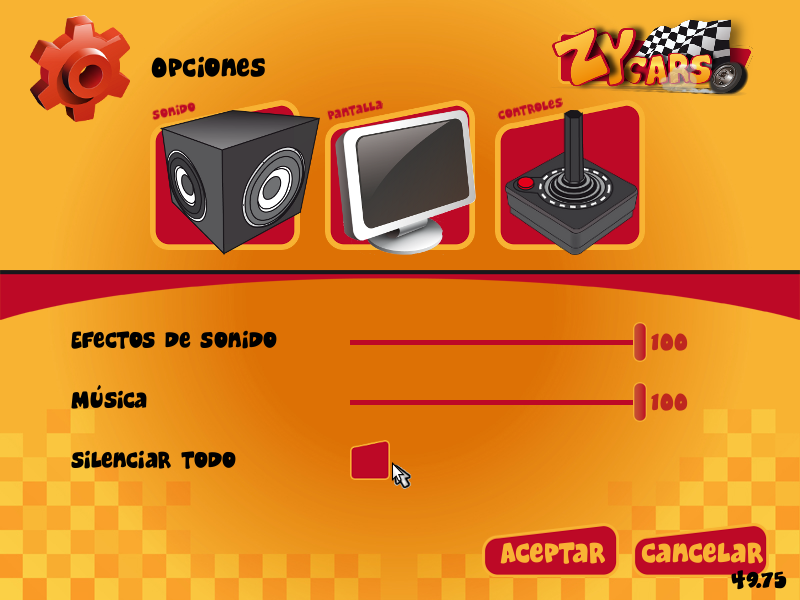
\includegraphics[scale=0.4]{imagenes/capturas/menuopcionesaudio.png}
  \end{center}
 \caption{Manual de usuario: Menú opciones - Audio}
\end{figure}

\paragraph{}
Como podemos ver, hay dos slider para la regulación del sonido y la música. También hay un checkbox, que nos permitirá silenciar todo, tanto 
los efectos de sonido como la música.

\subsection{Pantalla}

\paragraph{}
En este apartado solo dispondremos de una única opción. Esta opción nos permitira indicar si deseamos el juego a pantalla 
completa o si por el contrario lo deseamos al tamaño original de 800x600 píxeless.

\begin{figure}[H]
  \label{menu_pantalla}
  \begin{center}
    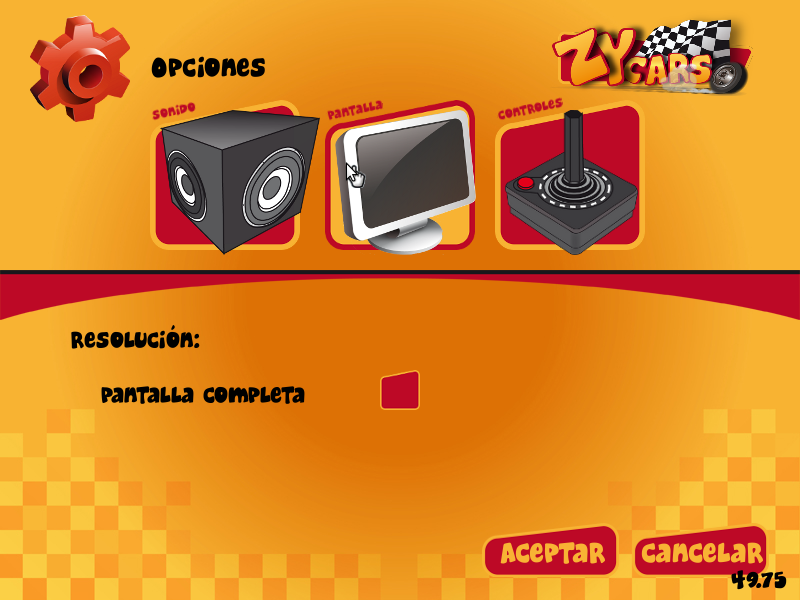
\includegraphics[scale=0.4]{imagenes/capturas/menuopcionespantalla.png}
  \end{center}
 \caption{Manual de usuario: Menú opciones - Pantalla}
\end{figure}

\subsection{Controles}

\paragraph{}
En esta sección del Menú de opciones podemos modificar que controles deseamos a la hora de manejar el vehículo. Los 
controles que podemos modificar son los de dirección, lanzamiento de los items y pausar el juego.

\begin{figure}[H]
  \label{menu_controles}
  \begin{center}
    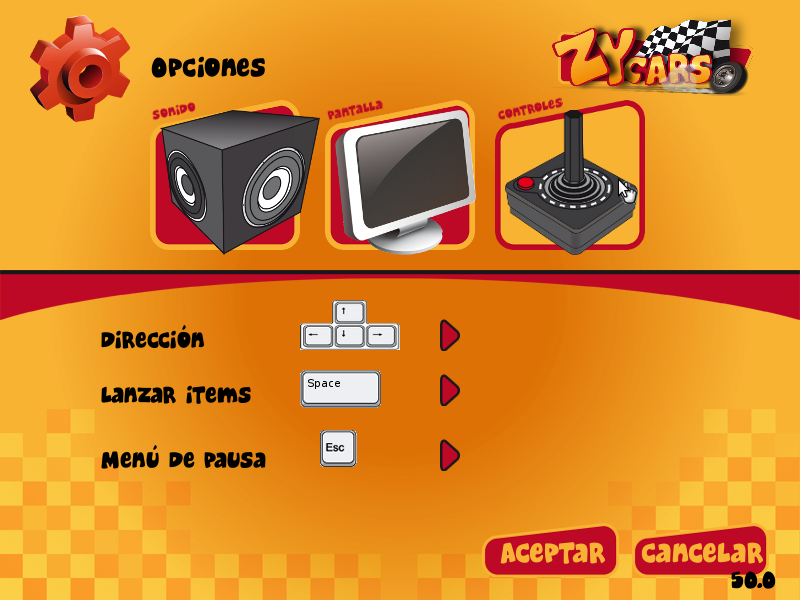
\includegraphics[scale=0.4]{imagenes/capturas/menuopcionescontroles.png}
  \end{center}
 \caption{Manual de usuario: Menú opciones - Controles}
\end{figure}

Debemos pulsar sobre las flechas para modificar los controles que queremos usar.

\section{Items}

\paragraph{}
Durante las carreras en las que compitamos contra la máquina, a lo largo de los circuitos encontraremos unas bolas que nos
proporionarán distintos elementos con los que podremos atacar a nuestros oponentes, dejar obstáculos o aumenten nuestra velocidad
durante un periodo de tiempo.

\begin{figure}[H]
  \label{caja_item}
  \begin{center}
    
\includegraphics[scale=1]{imagenes/items/item_box.png}
  \end{center}
 \caption{Manual de usuario: Bola de item.}
\end{figure}

\paragraph{}
Los distintos item que podemos conseguir tras atravesar la bola de item se describen a continuación:

\begin{itemize}
    \item \textbf{Misil}: este item proporciona un único misil al jugador, el cual podremos lanzar a nuestros competidores,
    en caso de que el misil colisione con algún jugador, este perdera el control durante unos instantes. En el caso de que el 
    misil colisione con algún objeto colisionable explotará.
        \begin{figure}[H]
          \label{misil}
          \begin{center}
            
\includegraphics[scale=1]{imagenes/items/missile.png}
          \end{center}
         \caption{Manual de usuario: Misil.}
        \end{figure}
        
    \item \textbf{Misil x 3}: este item nos proporciona 3 misiles que tienen las mismas características que el misil normal, 
    introducido anteriormente.
        \begin{figure}[H]
          \label{tres_misiles}
          \begin{center}
            
\includegraphics[scale=1]{imagenes/items/3missile.png}
          \end{center}
         \caption{Manual de usuario: Tres misiles.}
        \end{figure}
        
    \item \textbf{Bola}: este item tiene las mismas características que un misil, la única diferencia existente es que al 
    colisionar con algun objete no explotará, si no que rebotará. Sólo explotará en el caso de que colisione con algún
    jugador.        
        \begin{figure}[H]
          \label{bola}
          \begin{center}
            
\includegraphics[scale=1]{imagenes/items/ball.png}
          \end{center}
         \caption{Manual de usuario: Bola.}
        \end{figure}
        
    \item \textbf{Chicle}: este item nos proporciona un chicle que al lanzarlo en el circuito, se pegará al asfalto de forma 
    permanente. Cualquier jugador que pase por encima de él, decrementará su velocidad.
        \begin{figure}[H]
          \label{chicle}
          \begin{center}
            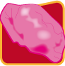
\includegraphics[scale=1]{imagenes/items/gum.png}
          \end{center}
         \caption{Manual de usuario: Chicle.}
        \end{figure}
        
    \item \textbf{Mancha de aceite}: este item nos proporciona una mancha de aceite que al lanzarla quedará en el circuito y 
    cualquier jugador que pase por encima, perdera el control del vehículo durante unos instantes.
        \begin{figure}[H]
          \label{mancha_aceite}
          \begin{center}
            
\includegraphics[scale=1]{imagenes/items/oil.png}
          \end{center}
         \caption{Manual de usuario: Macha de aceite.}
        \end{figure}
    
    \item \textbf{Turbo}: este item nos permitirá doblar nuestra velocidad durante unos instantes.
        \begin{figure}[H]
          \label{turbo}
          \begin{center}
            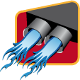
\includegraphics[scale=1]{imagenes/items/turbo.png}
          \end{center}
         \caption{Manual de usuario: Trubo.}
        \end{figure}
        
\end{itemize}

